\chapter{Ambiente di Analisi}
Al fine di osservare il comportamento del modulo SFA, e condurre l'analisi oggetto della Tesi, \`e stato costruito un ambiente atto a monitorare, in modo non intrusivo, il comportamento dell'algoritmo.\\*
L'ambiente di analisi \`e principalmente costituito dal software \emph{Rail Track Tool} (RTT).\\*
RTT simula l'architettura hardware descritta nel capitolo 2, ed incapsula come libreria il modulo SFA che viene eseguito bordo treno.
\section{Interfaccia utente}
All'avvio di RTT viene mostrata una finestra contenente l'interfaccia del software verso l'utente.
\begin{figure}[h]
	\centering
	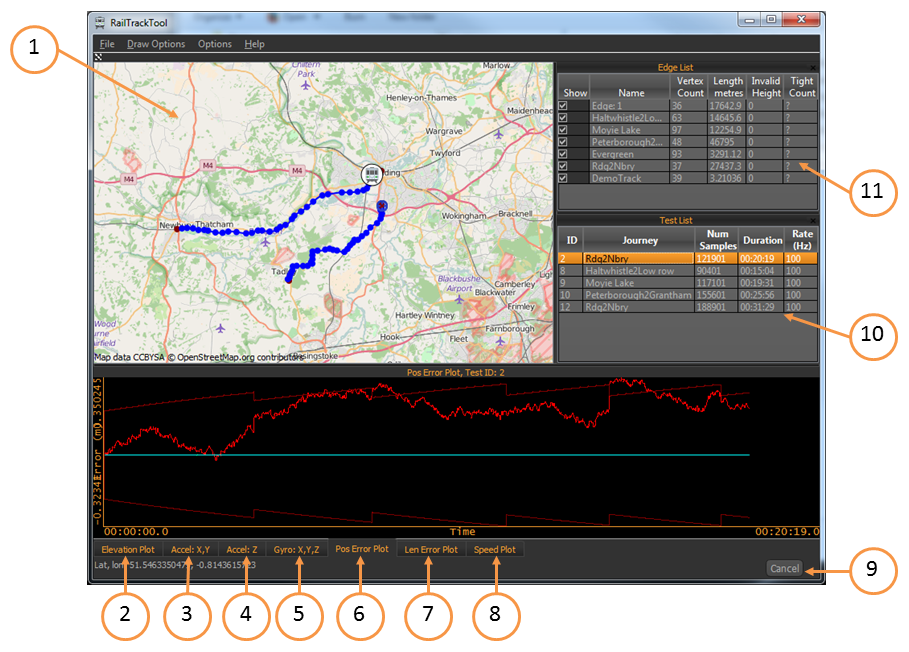
\includegraphics[height=8.2cm]{img/rtthci}
	\caption{Interfaccia RTT}
	\label{fig:rtt}
\end{figure}\newpage
Gli elementi che compongono tale interfaccia sono:
\begin{enumerate}
\item \texttt{Slippy map}: Mappa che visualizza le traccie memorizzate, all'interno delle quali verr\`a mostrata la posizione del treno durante l'esecuzione di SFA;
\item \texttt{Elevation plot}: Grafico che mostra l'altitudine della traccia in funzione della progressiva chilometrica della stessa;
\item \texttt{Accel X,Y}: Grafico delle misure dell'accelerometro fornite a SFA, relative agli assi normale e tangenziale alla traccia selezionata;
\item \texttt{Accel Z}: Grafico delle misure dell'accelerometro fornite a SFA, relative all'asse verticale alla traccia selezionata; 
\item \texttt{Gyro X,Y,Z}: Grafico delle misure del giroscopio fornite a SFA, relative agli assi normale, tangenziale e verticale alla traccia selezionata;
\item \texttt{Pos error plot}: Grafico che riporta, in funzione del tempo, la stima dell'errore commesso nel predire la posizione del treno;
\item \texttt{Len error plot}: Come \texttt{Pos error plot}, ma l'errore \`e espresso rispetto alla progressiva chilometrica e non rispetto al vettore posizione;
\item \texttt{Speed Plot}: Grafico che mostra la stima della velocit\`a del treno come funzione del tempo;
\item \texttt{Cancel button}: Pulsante da premere se si ha la necessit\`a di interrompere una simulazione;
\item \texttt{Test List}: Storico delle analisi effettuate;
\item \texttt{Edge List}: Lista delle tracce memorizzate.
\end{enumerate}
\section{Acquisizione delle misure}
Nel sistema reale le informazioni geografiche della traccia in esame sono salvate in un database caricato in memoria centrale. Nel contesto di analisi, queste informazioni sono stoccate in un database \emph{MySql} verso il quale si interfaccia RTT.\\*
Lo schema di tale database, identico al database utilizzato nel sistema reale, \`e mostrato in figura \ref{fig:splinedb}.\\*
\begin{figure}[h]
	\centering
	\includegraphics[scale=0.5]{../Trainpositioning/train-positioning-tools/Documentation/SplineDatabaseSchema}
	\caption{Schema database tracce}
	\label{fig:splinedb}
\end{figure}
Esso ha lo scopo di memorizzare, per ciascuna traccia, le coordinate geografiche dei suoi \emph{nodi}.\\*
Questa scelta \`e motivata dal fatto che una traccia viene modellata da SFA come una \emph{spline} interpolante i nodi scelti dall'utente sulla traccia stessa.\\*
Il meccanismo messo a disposizione da RTT per monitorare SFA include la possiblit\`a di generare automaticamente le misurazioni che verosimilmente si otterrebbero sul campo, date le caratteristiche della traccia e dei sensori utilizzati. All'atto di generazione delle misure, RTT interroga il database delle tracce per ottenere le informazioni necessarie a generare misure coerenti con la traccia in esame. Le misure vengono fornite a SFA attraverso le \texttt{API} del modulo che lo implementa, identiche a quelle invocate dal sistema reale.
\section{Monitoring}
Tramite un'apposita interfaccia interna a RTT, l'utente ha la possibilit\`a di definire le caratteristiche dei sensori, come mostrato nelle figure \ref{fig:datagenerationconfig} e \ref{fig:imuconfig}. Definiti i parametri di configurazione \`e possibile selezionare una traccia, e simulare l'esecuzione di SFA.\\* Durante la simulazione, la posizione del treno stimata dall'algoritmo verr\`a visualizzare sulla mappa. 
\begin{figure}[h]
	\centering
	\includegraphics[width=0.7\linewidth]{../Trainpositioning/train-positioning-tools/Documentation/UserGuide/DataGenerationConfig}
	\caption{Pannello di configurazione per generatore IMU}
	\label{fig:datagenerationconfig}
\end{figure}
\begin{figure}[h]
	\centering
	\includegraphics[width=0.7\linewidth]{../Trainpositioning/train-positioning-tools/Documentation/UserGuide/SensorModelConfig}
	\caption{Pannello di configurazione sensore inerziale}
	\label{fig:imuconfig}
\end{figure}
\newpage
Sui grafici nel pannello inferiore \`e possibile inoltre visualizzare i dati IMU forniti in ingresso all'algoritmo, l'errore commesso dallo stesso e la stima della velocit\`a del treno.\\*
\begin{figure}[h]
	\centering
	\includegraphics[width=0.8\linewidth]{../Trainpositioning/train-positioning-tools/Documentation/UserGuide/DataPlotImuAccel.png}
	\caption{Grafico valori di accelerazione assi X e Y}
	\label{fig:imuxy}
\end{figure}
\begin{figure}[h]
	\centering
	\includegraphics[width=0.8\linewidth]{../Trainpositioning/train-positioning-tools/Documentation/UserGuide/DataPlotImuGyro.png}
	\caption{Grafico valori di velocit\`a angolare}
	\label{fig:gyroxyz}
\end{figure}
\begin{figure}[h]
	\centering
	\includegraphics[width=0.7\linewidth]{../Trainpositioning/train-positioning-tools/Documentation/UserGuide/DataPlotPosError.png}
	\caption{Grafico errore sulla stima della posizione}
	\label{fig:dataplotposerror}
\end{figure}
\begin{figure}[h]
	\centering
	\includegraphics[width=0.7\linewidth]{../Trainpositioning/train-positioning-tools/Documentation/UserGuide/DataPlotLenError.png}
	\caption{Grafico errore sulla stima della progressiva chilometrica}
	\label{fig:dataplotlenerror}
\end{figure}
\begin{figure}[h]
	\centering
	\includegraphics[width=0.7\linewidth]{../Trainpositioning/train-positioning-tools/Documentation/UserGuide/DataPlotSpeed.png}
	\caption{Grafico della velocit\`a del treno stimata dall'algoritmo}
	\label{fig:dataplotspeed}
\end{figure}\clearpage
In fase di monitoring, RTT sfrutta le \texttt{API} del modulo SFA per ricevere le informazioni in uscita dall'algoritmo.\\*
Tali informazioni non sono esclusivamente limitate alla stima della posizione. Infatti il particolare SFA implementato in quest'applicazione, \`e in grado di stimare lo stato del treno sia in termini di posizione che in termini di velocit\`a. Per quanto concerne la stima degli errori commessi, l'algoritmo scelto calcola tali grandezze per definizione. \cite{librokalman}\\*
Non occorre quindi modificare il codice del modulo SFA per ottenere le informazioni interessanti ai fini dell'analisi.\\*
Al termine di ciascuna simulazione, RTT produce un report \texttt{HTML} contenente una sintesi dei risultati ottenuti.
